\seccion{Probabilidades}
\label{s:MP:Probabilidad}

El  concepto  de  {\it  probabilidad}  es importante  en  situaciones  donde  el
resultado (o {\it outcome}) de un  dado proceso o medici\'on es incierto, cuando
la salida de una experiencia no  es totalmente previsible. La probabilidad de un
evento es una medida que se asocia con cu\'an probable es el evento o resultado.

Una  definici\'on de  probabilidad puede  obtenerse en  base a  la enumeraci\'on
exhaustiva de los resultados posibles de un experimento o proceso,
%lo que no siempre es factible
suponiendo que el conjunto de posibilidades es completo en el sentido de que una
de  ellas debe ser  verdad. Si  el proceso  tiene $K$  resultados distinguibles,
mutuamente  excluyentes e  igualmente probables  (esto  es, no  se prefiere  una
posibilidad frente a  otras), y si $k$  de esos $K$ tienen un  dado atributo, la
probabilidad asociada a dicho atributo en un dado procesos es $\frac{k}{K}$. Por
ejemplo, sorteando un n\'umero entre los  naturales del 1 al 10, la probabilidad
de ``obtener un n\'umero par'' es $\frac5{10} = \frac12$.

Otra  definici\'on  de  probabilidad  se  basa  en  la  frecuencia  relativa  de
ocurrencia  de  un evento.   Si  en  una cantidad  $K$  muy  grande de  procesos
independientes  cierto   atributo  aparece  $k$   veces,  se  identifica   a  la
probabilidad  asociada a  un  proceso o  ensayo  con la  frecuencia relativa  de
ocurrencia    $\frac{k}{K}$    del    atributo~\cite[\&   Ref.]{Bra76,    Hal90,
  ShaVov06}~\footnote{A pesar de que la  noci\'on de azar (viniendo del arabe) o
  de alea (en  latin) es muy antiguo, el matem\'atico  y jugador (dados, cartas)
  italiano  Gerolamo Cardano es  ``probablemente'' un  de los  primeros tratando
  matematicamente del concepto  de probabilidad en el siglo  XVI, escribiando un
  libro sobre  los juegos  de azar en  1564 pero publicado  en 1663~\cite{Car63}
  (ver  tambi\'en~\cite{Bel05}  o~\cite[Cap.~4]{Hal90}).   Entre  los  numerosos
  matematicos desarollando  la teoria de  las probabildades, (en  particular los
  franceses  Pierre  de Fermat  y  Blaise  Pascal~\cite[Cap.~5]{Hal90}) hay  que
  mencionar   el   suizo  Jacob   Bernoulli   (miembro   de   una  dinastia   de
  m\'atematicos!)~\cite[en      latin]{Ber1713}      o~\cite{Ber1713:2},      el
  franco-ingl\'es Abraham  de Moivre~\cite{Dem56}, el franc\'es  Pierre Simon de
  Laplace~\cite{Lap20} quizas un de  los primeros llevandos un aporte importante
  al desarollo  de la  teoria de  las probabilidades en  los siglos  XVIII-XIX a
  trav\'es  de  este  punto  de  vista  ``frequencista''  y  combinatorial  (ver
  tambi\'en~\cite[Cap.~13, 15 \&~22]{Hal90}).}.
%lim N->infty n/N indef.

Los axiomas de Kolmogorov~\footnote{Un paso importante es debido a Kolmogorov en
  1933  que  se apoy\'o  sobre  trabajos  de  Richard von  Mises~\cite{Mis32}  y
  tambi\'en sobre  la teoria de  la medida y  de la integraci\'ion  debido entre
  otros a Emile Borel y Henri-L\'eon Lebesgues~\cite{Bor98, Bor09, Leb04, Leb18,
    Hal50}    para    formalizar    anal\'iticamente    la   teoria    de    las
  probabilidades~\cite{Kol56, BarNov78,   JacPro03}.}    proveen   requisitos
suficientes  para  determinar completamente  las  propiedades  de  la medida  de
probabilidad $P(A)$  que se puede asociar a  un evento $A$ entre  un conjunto de
resultados o eventos de un proceso.

Llamemos $\Omega$ al {\it espacio  muestral} o {\it espacio fundamental}, que es
el espacio de  {\it muestras (outcomes en ingl\'es)} \  $\omega \in \Omega$.  Se
asocia \ $\A$ \ una colecci\'on  de conjuntos de \ $\Omega$, donde los elementos
de $\A$ son llamados {\it eventos}.
% total de eventos.
Por ejemplo, $\Omega$ puede  ser las caras de un dado de  6 caras (los n\'umeros
naturales del 1 al  6, o las letras {\it a, b, c, d,  e, f}, u otro etiquetado),
$\A$ teniendo los eventos
% si $A$ es el evento
$A$ ``es  un n\'umero  natural par''  y $B$ indicando  ``es un  n\'umero natural
impar''.
% ,  el espacio  muestral  $\Omega  = \{  A  , B  \}$  indica  ``es un  n\'umero
% natural'';
En el caso de analizar el tiempo de vida de un aparato, $\Omega \equiv \Rset_+$.
% en el  lanzamiento de un  dado de 6  caras es $\Omega$  es el conjunto  de las
% etiquetas que se asigne a cada una de las caras (los n\'umeros naturales del 1
% al 6, o las letras {\it a, b, c, d, e, f}, u otro etiquetado).
El  conjunto  de  resultados  posibles  se  supone  conocido,  a\'un  cuando  se
desconozca de antemano el resultado de una prueba.

Entre  los eventos  se  pueden considerar  operaciones  an\'alogas a  las de  la
teor\'ia de  conjuntos (ej.~\cite{Spi76,  Bre88, ManWol95, Sie75,  Sie76, Bor98,
  Bor09}):
%
\begin{itemize}
\item Combinaci\'on  o uni\'on de  eventos: \ $A  \cup B$, implicando que  se da
  $A$, \'o $B$, o ambos (ej. por  un dado, $A$ eventos ``cara par'' y $B$ evento
  ``cara menor o igual a 3'' tal que $A \cup B = \{1 \, , \, 2 \, , \, 3 \, , \,
  4 \,  , \, 6\}$); Seg\'un la  literatura, se denota a  veces \ $A+B$ \  o \ $A
  \wedge B$.
%
\item  Intersecci\'on de  eventos:  \ $A\cap  B$,  implicando que  se dan  ambos
  $A$~y~$B$ (con  el ejemplo precediente,  $A \cap  B = \{  2 \}$); Se  denota a
  veces \ $(A,B)$ \ o \ $A \vee B$.
%
\item Complemento de un evento: \ $\bar{A}$ e indica que no se da $A$; Se denota
  a veces \ $-A$  \ o \ $A^c$ (con el ejemplo precediente, $\bar{A}  = \{ 1 \, ,
  \, 3 \, , \, 5 \}$).
%
\item  Eventos  {\it  disjuntos}  o   {\it  mutuamente  excluyentes}  o  {\it  o
    incompatibles}: \ son aquellos que no se  superponen, se anota \ $A \cap B =
  \emptyset$  \ donde  \  $\emptyset =  \bar{\Omega}$  \ denota  el evento  nulo
  (evento que no  puede ocurrir, es el complemento de  $\Omega$, por ejemplo $A$
  ``cara par'' y $B$ ``cara impar'').
%
\item \modif{Denotaremos  tambi\'en $A \backslash B$  \ cuando el  evento $A$ se
    realiza pero  no $B$;  A veces,  se lo denota  tambi\'en \  $A-B$, \  que es
    tambi\'en \  $A \cap \bar{B}$, por  ejemplo ``cara par'' y  $B$ ``cara menor
    que 3''.}
\end{itemize}
%
\noindent Eso es ilustrado en la figura Fig.~\ref{fig:MP:Ensembles} \modif{en lo
  que es  conocido como diagrama de Venn~\footnote{\modif{Este  tipo de diagaram
      fue  popularizado por  el ingles  J.  M.   A.  Venn  en 1880,  pero  en su
      papel~\cite{Ven80} da la partenidad  al matem\'atico suizo Leohnard Euler,
      un de  los primeros a usar tal  representaci\'on en el siglo  XVIII en sus
      cartas a una  princesa alemana (ver~\cite[L~102-105, pp.~95-126]{Eul68}) o
      antes a Christian Weise y Johan Christian Langius~\cite{Lan12}; apareci\'o
      a\'un  en trabajos  de  Leibniz en  el  siglo anterio.}}}.   La uni\'on  e
intersecci\'on satisfacen a  las mismas reglas que en  la teoria ensemblista, es
decir cada una es comutativa \ $A \cup B = B \cup A$, \ $A \cap B = B \cap A$, \
asociativa \ $(A \cup B)  \cup C = A \cup (B \cup C)$, \ $(A  \cap B) \cap C = A
\cap (B \cap C)$, \ distributiva con respeto a la otra \ $(A \cup B) \cap C = (A
\cap C) \cup (B \cap C)$ \ y \ $(A  \cap B) \cup C = (A \cup C) \cap (B \cup C)$
\  (ver  ej.~\cite{Jef48,  Jef73,   Hal50,  Fel71,  Bre88,  ManWol95,  IbaPar97,
  LehCas98, AthLah06, Coh13, HogMck13}).

\begin{figure}[h!]
\begin{center} 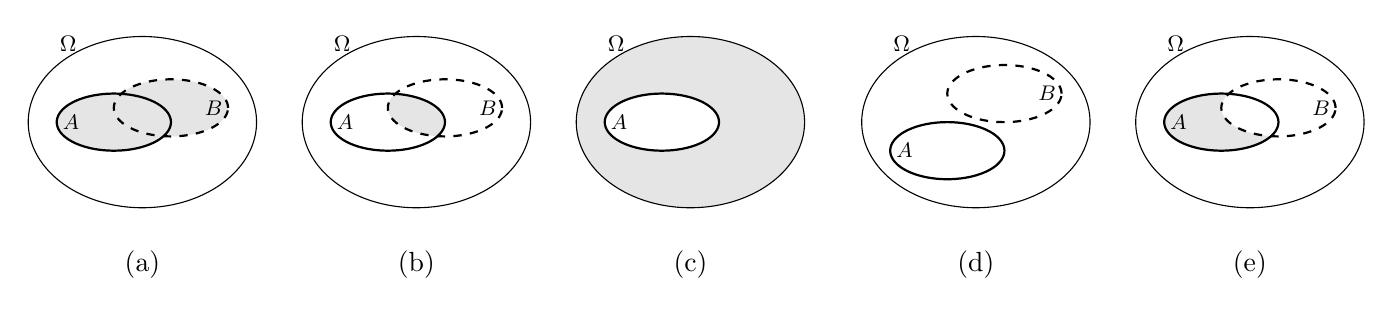
\begin{tikzpicture}[scale=.725]
\shorthandoff{>}
%
% Union y interseccion:
%
% Omega: .25*(x-.25)^2 + (y/1.5)^2 = 1
% A: x^2 + 4 y^2 = 1
% B: (x-1)^2 + 4 (y-1/4)^2 = 1
% A y B se cruzan cuando x = 1 \pm sqrt(55)/10 =>
% theta = acos(.5 \pm sqrt(55)/20) para A
% theta = acos(-.5 \pm sqrt(55)/20) para A
\pgfmathsetmacro{\s}{acos(.5-sqrt(55)/20)};
\pgfmathsetmacro{\t}{-acos(.5+sqrt(55)/20)};
\pgfmathsetmacro{\u}{-acos(-.5+sqrt(55)/20)};
\pgfmathsetmacro{\v}{acos(-.5-sqrt(55)/20)-360};
%
%
%Union
\begin{scope}
%
\fill[opacity=.1]
plot[domain=\s:\t+360,samples=200] ({cos(\x)},{.5*sin(\x)})
-- plot[domain=\u:\v+360,samples=200] ({cos(\x)+1},{.5*sin(\x)+.25})
-- cycle;
%
% borders A, B y Omega
\draw[domain=0:360,samples=200,thick] plot ({cos(\x)},{.5*sin(\x)});
\draw[dashed,domain=0:360,samples=200,thick] plot ({cos(\x)+1},{.5*sin(\x)+.25});
\draw[domain=0:360,samples=200] plot ({2*cos(\x)+.5},{1.5*sin(\x)});
%
% A, B, Omega
\draw (-.75,0) node[scale=.85]{\small $A$};
\draw(1.75,.25) node[scale=.85]{\small $B$};
\draw(-.5,1.375) node[left,scale=.9]{\small $\Omega$};
%
\draw (.5,-2.5) node{(a)};
\end{scope}
%
%
% Interseccion
\begin{scope}[xshift=4.8cm]
%
\fill[opacity=.1]
plot[domain=\s:\t,samples=200] ({cos(\x)},{.5*sin(\x)})
-- plot[domain=\u:\v,samples=200] ({cos(\x)+1},{.5*sin(\x)+.25})
-- cycle;
%
% borders A, B y Omega
\draw[domain=0:360,samples=200,thick] plot ({cos(\x)},{.5*sin(\x)});
\draw[dashed,domain=0:360,samples=200,thick] plot ({cos(\x)+1},{.5*sin(\x)+.25});
\draw[domain=0:360,samples=200] plot ({2*cos(\x)+.5},{1.5*sin(\x)});
%
% A, B, Omega
\draw (-.75,0) node[scale=.85]{\small $A$};
\draw(1.75,.25) node[scale=.85]{\small $B$};
\draw(-.5,1.375) node[left,scale=.9]{\small $\Omega$};
%
\draw (.5,-2.5) node{(b)};
\end{scope}
%
%
% Complemento
\begin{scope}[xshift=9.6cm]
%
\fill[opacity=.1]
plot[domain=0:360,samples=200] ({2*cos(\x)+.5},{1.5*sin(\x)})
-- plot[domain=0:360,samples=200] ({cos(\x)},{-.5*sin(\x)})
-- cycle;
%
% borders A y Omega
\draw[domain=0:360,samples=200,thick] plot ({cos(\x)},{.5*sin(\x)});
\draw[domain=0:360,samples=200] plot ({2*cos(\x)+.5},{1.5*sin(\x)});
%
% A, Omega
\draw (-.75,0) node[scale=.85]{\small $A$};
\draw(-.5,1.375) node[left,scale=.9]{\small $\Omega$};
%
\draw (.5,-2.5) node{(c)};
\end{scope}
%
%
% Excluyentes
\begin{scope}[xshift=14.6cm]
%
% borders A, B (con un shift...) y Omega
\draw[domain=0:360,samples=200,thick] plot ({cos(\x)},{.5*sin(\x)-.5});
\draw[dashed,domain=0:360,samples=200,thick] plot ({cos(\x)+1},{.5*sin(\x)+.5});
\draw[domain=0:360,samples=200] plot ({2*cos(\x)+.5},{1.5*sin(\x)});
%
% A, B, Omega
\draw (-.75,-.5) node[scale=.85]{\small $A$};
\draw (1.75,.5) node[scale=.85]{\small $B$};
\draw(-.5,1.375) node[left,scale=.9]{\small $\Omega$};
%
\draw (.5,-2.5) node{(d)};
\end{scope}
%
%
% privado
\begin{scope}[xshift=19.4cm]
%
\fill[opacity=.1]
plot[domain=\s:\t+360,samples=200] ({cos(\x)},{.5*sin(\x)})
-- plot[domain=\u:\v,samples=200] ({cos(\x)+1},{.5*sin(\x)+.25})
-- cycle;
%
% borders A, B y Omega
\draw[domain=0:360,samples=200,thick] plot ({cos(\x)},{.5*sin(\x)});
\draw[dashed,domain=0:360,samples=200,thick] plot ({cos(\x)+1},{.5*sin(\x)+.25});
\draw[domain=0:360,samples=200] plot ({2*cos(\x)+.5},{1.5*sin(\x)});
%
% A, B, Omega
\draw (-.75,0) node[scale=.85]{\small $A$};
\draw(1.75,.25) node[scale=.85]{\small $B$};
\draw(-.5,1.375) node[left,scale=.9]{\small $\Omega$};
%
\draw (.5,-2.5) node{(e)};
\end{scope}
%
\end{tikzpicture} \end{center}
%
\leyenda{Ilustraci\'on   de  la  operaciones   de  uni\'on   $A  \cup   B$  (a),
  intersecci\'on $A \cap B$  (b), complemento $\bar{A}$ (c), eventos excluyentes
  $A \cap B =  \emptyset$ (d), \ y $A \backslash B$  (e). $A$ es representado en
  linea  llena, $B$  en linea  discontinua; (a)-(c)  y (e),  el resultado  de la
  operaci\'on es la zona en grise.}
% A veces, esta representaci\'on ensemblista se
%  denota {\it diagrama de Venn o de Euler~\protect\footnotemark}}
\label{fig:MP:Ensembles}
\end{figure}
% \footnotetext{\modif{Este tipo de diagaram  fue popularizado por Venn, pero en
%     su papel~\cite{Ven} da la partenidad al matem\'atico aleman E. Euler un de
%     los primeros a usar tal representaci\'on, en el siglo XVI~\cite{Eul}.}}

Formalmente, se define  de manera abstracta un espacio  medible $(\Omega,\A)$ de
la  manera  siguiente~\cite{Hal50,  Fel68,  Fel71,  Bre88,  IbaPar97,  AthLah06,
  Bog07:v1, Coh13} (ver  tambi\'en~\cite[\& Ref.]{BarNov78, Bor98, Sie18, Sie75,
  Sie76} para notas hist\'oricas):
%
\begin{definicion}[Espacio medible]
  $(\Omega, \A)$ \ formado de un espacio muestral \ $\Omega$ \ y una colecci\'on
  \ $\A$  \ de conjuntos  de \  $\Omega$ \ es  llamado {\it espacio  medible} si
  satisface a los requisitos
  %
  \begin{enumerate}%[label={(\Roman*)}]
  \item $\emptyset \in \A$,
  %
  \item si $A \in \A$, entonces \ $\bar{A} \in \A$,
  %
  \item la uni\'on numerable de conjuntos de $\A$ queda en $\A$ ($\A$ es cerrado
    por la un\'ion numerable).
  %
  \end{enumerate}
  %
  Con estas propiedades, $\A$ es llamado {\it $\sigma$-\'algebra}. Los elementos
  de $\A$ son dichos {\it medibles}.
\end{definicion}
%
\noindent Es  sencillo mostrar de  que $\Omega$ tambi\'en  es en $\A$, y  de que
$\A$   est   cerrado  por   la   intersecci\'on   numerable.    Un  ejemplo   de
$\sigma$-\'algebra sobre \ $\Omega = \{ 1 \, , \,  2 \, , \, 3 \, , \, 4 \, , \,
5 \, , \, 6 \}$ \ puede ser \ $\big\{ \emptyset \, , \, \Omega \, , \, \{ 1 \, ,
\, 2 \, , \, 3 \} \, , \, \{ 4 \, , \, 5 \, , \, 6 \} \big\}$.

\modif{Saliendo de \ $(\Omega,\A)$, \  se asocia una noci\'on de probabilidad} \
$P$ \ de un dado evento quedan determinadas por los siguientes \modif{requisitos
  llamados  {\it  Axiomas  de  Kolmogorov}} (ej.~\cite{Spi76,  Kol56,  ShaVov06,
  Pla05}):
%\noindent {\it Axiomas de Kolmogorov}
%
\begin{enumerate}
\item $P(A_i) \geq 0 \ \ \forall \ A_i \A$
%
\item  Si $\{ A_i  \}_i$ son  eventos mutuamente  excluyentes de  $\A$, entonces
  $\displaystyle P\left( \bigcup_i A_i \right) = \sum_i P(A_i)$
%
\item $P(\Omega) = 1$
\end{enumerate}
%
\modif{M\'as f}ormalmente,  se define  un {\it espacio  de probabilidad}  o {\it
  espacio  probabil\'istico} de la  manera siguiente~\cite{Hal50,  Fel68, Fel71,
  Bre88, IbaPar97, AthLah06, Bog07:v1, JacPro03, Coh13}:
%
\begin{definicion}[Espacio de medida y espacio probabil\'istico]
  Sea $(\Omega,\A)$ un espacio medible.  Una funci\'on $\mu: \A \mapsto \Rset_+$
  tal que
  %
  \begin{enumerate}
  \item $\mu(\emptyset) = 0$, y
  \item para  cualquier conjunto numerable  $\{ A_i \}$ de  elementos mutuamente
    excluyentes  de $\A$  se tiene  $\mu\left(  \bigcup_i A_i  \right) =  \sum_i
    \mu(A_i)$
  \end{enumerate}
  %
  es  llamada {\it  funci\'on  medida}  o {\it  medida  $\sigma$-aditiva} y  el
  espacio $(\Omega,\A,\mu)$ es  llamado {\it espacio de medida}.

  Cuando $\mu$  es acotada por  arriba, $\mu(\Omega) <  + \infty$, la  medida es
  dicha  {\it  finita} y  el  espacio tambi\'n  es  dicho  finito. Adem\'as,  si
  \[ P \equiv  \mu, \quad P(\Omega) = 1,  \] la medida es dicha  medida de {\it
    probabilidad}, $\mu \equiv P$.  En  este caso, el espacio $(\Omega,\A,P)$ es
  llamado {\it espacio probabil\'istico}.
\end{definicion}
%
\noindent  (ver tambi\'en~\cite[Cap.~5  \&  6]{KolFom61}). \modif{Es  importante
  notar de  que una  combinaci\'on lineal positiva  de medida queda  una medida,
  pero el producto de dos medidas no es una medida mas.}

A  partir de  los axiomas  de Kolmogorov  se pueden  probar varios  corolarios y
propiedades:
%
\begin{itemize}
\item la probabilidad de un evento seguro o cierto es 1;
%
\item  la   probabilidad  de   un  evento   que  no  puede   ocurrir  es   0:  \
  \modif{entre otros,} \ $P(\emptyset) = 0$;
%
\item el rango  de las probabilidades est\'a  acotado: \ $0 \leq P(A)  \leq 1\ \
  \forall \ A \in \A$;
%
\item condici\'on de  normalizaci\'on: \ si $\Omega =  \bigcup_{i=1}^n A_i$, con
  $A_i$  mutuamente  excluyentes,  entonces  \  $\sum_{i=1}^n P(A_i)  =  1$;  el
  conjunto  $\{ A_i  \}_{i=1}^n$  es  dicho {\it  conjunto  completo de  eventos
    posibles      excluyentes      entre      s\'i}     y      es      ilustrado
  figure~\ref{fig:MP:CompletoSub};
%
\item si $A$ es subconjunto de $B$,  lo que escribiremos $A \subset B$, es decir
  si  $B$  se realiza,  $A$  se realiza  tambi\'en  (pero  no necesariamente  al
  rev\'es),     entonces     \     $P(A)     \leq    P(B)$;     es     ilustrado
  figure~\ref{fig:MP:CompletoSub};
\end{itemize}

\begin{figure}[h!]
\begin{center} 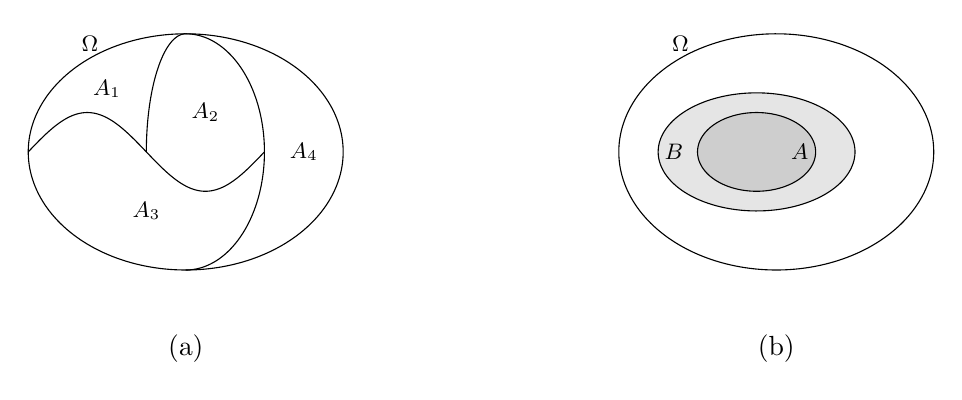
\begin{tikzpicture}%[scale=.9]
\shorthandoff{>}
%
% Particion
\begin{scope}
%
% Omega y A_i
\draw[domain=0:360,samples=200] plot ({2*cos(\x)+.5},{1.5*sin(\x)});
\draw[domain=-90:90,samples=200] plot ({cos(\x)+.5},{1.5*sin(\x)});
\draw[domain=90:180,samples=200] plot ({.5*cos(\x)+.5},{1.5*sin(\x)});
\draw[domain=0:3,samples=200] plot (\x-1.5,{.5*sin(120*\x)});
%
%
% Omega y A_i's
\draw(-.5,1.375) node[left,scale=.9]{\small $\Omega$};
\draw(-.5,.8) node[scale=.9]{\small $A_1$};
\draw(.75,.5) node[scale=.9]{\small $A_2$};
\draw(0,-.75) node[scale=.9]{\small $A_3$};
\draw(2,0) node[scale=.9]{\small $A_4$};
%
\draw (.5,-2.5) node{(a)};
\end{scope}
%
%
% Inclusion
\begin{scope}[xshift=7.5cm]
%
\fill[opacity=.1] plot[domain=0:360,samples=200] ({1.25*cos(\x)+.25},{.75*sin(\x)});
\fill[opacity=.1] plot[domain=0:360,samples=200] ({.75*cos(\x)+.25},{.5*sin(\x)});
%
% borders A, B y Omega
\draw[domain=0:360,samples=200] plot ({1.25*cos(\x)+.25},{.75*sin(\x)});
\draw[domain=0:360,samples=200] plot ({.75*cos(\x)+.25},{.5*sin(\x)});
\draw[domain=0:360,samples=200] plot ({2*cos(\x)+.5},{1.5*sin(\x)});
%
% A, B, Omega
\draw(.8,0) node[scale=.9]{\small $A$};
\draw (-.8,0) node[scale=.9]{\small $B$};
\draw(-.5,1.375) node[left,scale=.9]{\small $\Omega$};
%
\draw (.5,-2.5) node{(b)};
\end{scope}
%
\end{tikzpicture} \end{center}
%
\leyenda{Ilustraci\'on  de  conjunto completo  de  eventos posibles  excluyentes
  entre s\'i  (a), y de  la inclusi\'on  (b) donde $A$  es en grise  (claro como
  oscuro) mientras de que $B$ es en grise oscuro.}
\label{fig:MP:CompletoSub}
\end{figure}

Nota:  la probabilidad  \ $P(A  \cap B)$  \ del  evento $A  \cap B$  \  se llama
tambi\'en {\it probabilidad conjunta} de \ $A$ \ y \ $B$.
%$P(A  \cap B)  = P(B  \cap A)$}  es la
%probabilidad del evento conjunto dado por  la composici\'on de los eventos $A$ y
%$B$. 

Se demuestra que
%
\begin{itemize}
\item $P(A  \cap B)$ est\'a acotada:  \ $0 \leq P(A  \cap B) \leq  \min\{ P(A) ,
  P(B)\}$; (viene de \ $A \cap B \subset A$ \ y \ $A \cap B \subset B$);
%
\item si  $A$ y $B$ son  mutuamente excluyentes, entonces  \ $p(A \cap B)  = 0$;
  (viene de \ $A \cap B = \emptyset$);
%
\item  si  $\{ B_j  \}_{j=1}^m$  es un  conjunto  completo  de eventos  posibles
  excluyentes entre s\'i, entonces \ $\sum_{j=1}^m P(A \cap B_j) = P(A)$; (viene
  de $\{  A \cap B_j \}_j$ mutuamente  excluyentes y \ $\bigcup_j  \left( A \cap
    B_j\right) = A \cap \left( \bigcup_j B_j \right) = A \cap \Omega = A$).
\end{itemize}

En el caso de eventos no necesariamente mutuamente excluyentes, se prueba que la
{\it ley de composici\'on} o {\it f\'ormula de inclusi\'on-exclusi\'on} es
%
\[
P(A \cup B) = P(A) + P(B) - P(A \cap B) \leq P(A) + P(B), 
\]
%
y que para $n$ eventos resulta
%
\[
P\left( \bigcup_{i=1}^n A_i \right) \leq \sum_{i=1}^n P\left( A_i \right).
\]
%
La  igualdad  vale  en  el  caso  especial  de  eventos  mutuamente  excluyentes
(recuperando el segundo axioma de Kolmogorov).

Se  prueba tambi\'en  de que  si $\{  A_i \}_{i=1}^{+\infty}$  es  una secuencia
creciente  de eventos,  \ie $\forall  \, i  \ge 1,  \quad A_i  \subset A_{i+1}$,
entonces
%
\[
P\left( \bigcup_{i=1}^{+\infty} A_i \right) = \lim_{i \to +\infty} P(A_i).
\]
%
Similarmente,  si $\{ A_i  \}_{i=1}^{+\infty}$ es  una secuencia  decreciente de
eventos, \ie $\forall \, i \ge 1, \quad A_{i+1} \subset A_i$, entonces
%
\[
P\left( \bigcap_{i=1}^{+\infty} A_i \right) = \lim_{i \to +\infty} P(A_i).
\]

Se puede preguntarse de cual es la probabilidad de un evento $A$, si sabemos que
tenemos un evento $B$, dado.  Por  ejemplo, por un dado de 6 caras equilibriado,
cual es la probabilidad de tener  un n\'umero par sabiendo que tenemos un numero
menor \modif{o} a  igual a 3.  La respuesta \modif{se  encuentra} en la noci\'on
de  {\it probabilidad condicional}~\cite{Hau01,  Jef48, Jef73,  Bre88, ManWol95,
  JacPro03, ShaVov06}:
%
\begin{definicion}[Probabilidad condicional]\label{def:MP:ProbaCondicional}
  \underline{Por definici\'on},  la {\it  probabilidad condicional} de  $A$ dado
  $B$ es la raz\'on entre la  probabilidad del evento conjunto y la probabilidad
  de  que se  d\'e $B$  (cuando \'este  es un  evento \modif{de  probabilidad no
    nula}):
  %
  \[
  P(A|B) = \frac{P(A \cap B)}{P(B)}.
  \]
\end{definicion}
%
En  el  ejemplo precediente,  la  probabilidad  va a  ser  $P(A|B)  = \frac13  =
\frac{\frac16}{\frac12}  = \frac{P(A  \cup B)}{P(B)}$. 

\modif{Claramente   del   hecho   de   que   \   $P$  \   es   una   medida   de
  probabilidad, \[P(A|B) \ge  0.\] Luego, de \  $A \cap B \subseteq B$  \ viene \
  $P(A \cap B) \le P(B)$, es decir  \ $P(A|B) \le 1$. Adem\'as, \ $P(\Omega \cap
  B) = P(B)$ \ dando \[P(\Omega|B) = 1.\] Para cualquier conjunto \ $\{ A_i \}$ \
  de eventos  mutuamente excluyentes, los  \ $\left( A_i  \cap B \right)$  \ son
  tambi\'en mutuamente  excluyentes, as\'i que \  $\displaystyle P\left( \left(
      \bigcup_i A_i  \right) \bigcap  B \right) =  P\left( \bigcup_i  \left( A_i
      \bigcap  B \right)  \right)  = \sum_i  P\left(  A_i \bigcap  B \right)$  \
  dando  \[P\left( \left.  \bigcup_i  A_i  \right| B  \right)  = \sum_i  P\left(
    \left. A_i \right| B \right).\] Dicho de otra manera,}
% y  que es
%aditiva  para  una  uni\'on  de  eventos  mutuamente  excluyentes  referidos  al
%cumplimiento de $B$.  Luego, 
$P(A|B)$ es una medida de  probabilidad~\footnote{Se puede definir un espacio de
  probabilidad $(  \Omega_B, \A_B  , P_B)$ donde  $P_B(A) \equiv  P(A|B)$.}; Por
eso, a  veces en la literatura  se la denota  $P_B(A)$ \ \modif{pero no  vamos a
  usar esta notaci\'on para no confundirla  con la medida de probabilidad de una
  variable  aleatoria  que definiremos  en  la  secci\'on siguiente}.   Diversas
situaciones  de  probabilidades  condicionales   son  ilustradas  en  la  figura
siguiente, Fig.~\ref{fig:MP:Condicional}.

\begin{figure}[h!]
\begin{center} 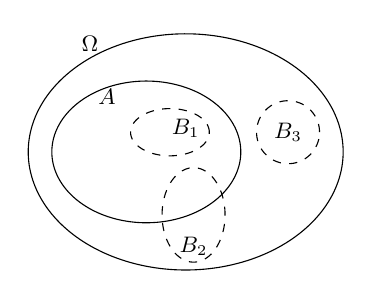
\begin{tikzpicture}%[scale=.9]
\shorthandoff{>}
%
\begin{scope}
%
% Omega, A, B_i
\draw[domain=0:360,samples=200] plot ({2*cos(\x)+.5},{1.5*sin(\x)});
\draw[domain=0:360,samples=200] plot ({1.2*cos(\x)},{.9*sin(\x)});
\draw[dashed,domain=0:360,samples=200] plot ({.5*cos(\x)+.3},{.3*sin(\x)+.25});
\draw[dashed,domain=0:360,samples=200] plot ({.4*cos(\x)+.6},{.6*sin(\x)-.8});
\draw[dashed,domain=0:360,samples=200] plot ({.4*cos(\x)+1.8},{.4*sin(\x)+.25});
%
%
% Omega y A_i's
\draw(-.5,1.375) node[left,scale=.9]{\small $\Omega$};
\draw(-.5,.7) node[scale=.9]{\small $A$};
\draw(.5,.3) node[scale=.9]{\small $B_1$};
\draw(.6,-1.2) node[scale=.9]{\small $B_2$};
\draw(1.8,.25) node[scale=.9]{\small $B_3$};
%
\end{scope}
%
\end{tikzpicture} \end{center}
%
\leyenda{Ilustraci\'on  de  la probabilidad  condicional  con  $A$ interior  del
  elipse  en linea  llena  y unos  $B_i$  interiores de  los  elipses en  lineas
  discontinuas.   \ $\omega  \in B_1  \Rightarrow \omega  \in A$  \ as\'i  que \
  $P(A|B_1) = 1$. Al rev\'es, \  $\omega \in B_3 \Rightarrow \omega \not\in A$ \
  as\'i que \  $P(A|B_3) = 0$.  Entre estas  situaciones extremas, si $P(\bar{A}
  \cap B_2)  \ne 0$ \ y  \ $P(A \cap  B_2) \ne 0$ \  tenemos $0 < P(A|B_2)  < 1$
  (ej.  con   probabilidades  iguales  a   las  superficias  relativas   de  los
  conjuntos).}
\label{fig:MP:Condicional}
\end{figure}

Algunas propiedades interesantes son las siguientes:
%
\begin{itemize}
  \modif{\item $P(A \cap B  | B) = P(A|B)$. \ Viene de $P(A \cap  B \cap B) = P(A
    \cap B)$;
%
\item si $A$ \ y \ $B$ \ son excluyentes, obviamente \ $P(A|B) = 0$;
%
\item si $B  \subseteq C$, entonces \ $P(A |  B \cap C) = P(A|B)$.  \ Viene de \
  $P(A |  B \cap C) =  \frac{P(A \cap B \cap  C)}{P(B \cap C)}  = \frac{P(A \cap
    B)}{P(B)}$ \ porque \ $B \cap C = B$;}
%
\item condici\'on  de normalizaci\'on: \  $\sum_{i=1}^n P(A_i|B) = 1$,  siendo \
  $\{ A_i \}_{i=1}^n$  \ un conjunto completo de  resultados posibles mutuamente
  excluyentes;
%
\item relaci\'on  entre probabilidades condicionales  inversas: \ $\displaystyle
  P(B|A)  = \frac{P(B)}{P(A)}  P(A|B)$, de  donde \  $p(A|B)$ \  y \  $p(B|A)$ \
  coinciden s\'olo cuando \ $A$ \ y \ $B$ \ tienen la misma probabilidad;
%
\item {\it f\'ormula de probabilidades totales}: \ si $\{ B_j \}$ es un conjunto
  completo de eventos no nulos mutuamente excluyentes, entonces
  %
  \[
  P(A) = \sum_j P(A|B_j) P(B_j);
  \]
  %
  viene de \ $A = A \cap  \left( \bigcup_j B_j \right) = \bigcup_j \left( A \cap
    B_j \right)$  \ donde  los \ $A  \cap B_j$  \ son mutuamente  excluyentes, y
  $P\left( A \cap B_j \right) = P(A|B_j) P(B_j)$;
%
\item {\it  f\'ormula de Bayes}:  \ si  $\{ B_j \}$  es un conjunto  completo de
  eventos no nulos mutuamente excluyentes, entonces
  %
  \[
  P(B_i|A) = \frac{P(A \cap B_i)}{P(A)} = \frac{P(A|B_i) P(B_i)}{\sum_j P(A|B_j)
    P(B_j)};
  \]
  %
  (ver~\cite{Bre88, JacPro03, Bay63, Bar58}).
\end{itemize}

Terminamos  esta   secci\'on  por  la   noci\'on  de  independencia   entre  dos
eventos. Por  ejemplo, si dos dados  son tirados sobre dos  mesas diferentes, no
hay ninguna raz\'on de  que la muestra de uno ``influye'' la  del otro. Dicho de
otra manera,  dos eventos son independientes  si conciendo uno  no lleva ninguna
``informaci\'on'' sobre el otro~\cite{Bre88, ManWol95, Hau01, JacPro03, Bor09}:
%
\begin{definicion}[Independencia estad\'istica]
  Dos eventos \ $A$ \ y \ $B$ \ se dicen {\it estad\'isticamente independientes}
  si la  probabilidad condicional  de $A$  dado $B$ es  igual a  la probabilidad
  incondicional de $A$:
  %
  \[
   P(A|B) = P(A).
   \]
  %
   Es equivalente al hecho de que la probabilidad conjunta se factoriza,
  %
  \[
   P(A \cap B) = P(A) P(B).
   \]
\end{definicion}
%
Por  inducci\'on, la  condici\'on necesaria  y suficiente  para que  $n$ eventos
$A_1,\ldots,A_n$ sean estad\'isticamente {\em mutuamente} independientes es que
la probabilidad conjunta se factorice como
%
\[
P\left( \bigcap_{i=1}^n A_i \right) = \prod_{i=1}^n P(A_i).
\]
%
Se  deduce que  los  eventos mutuamente  excluyentes  no son  estad\'isticamente
independientes.

Es importante notar  que la independencia mutua \underline{no  es equivalente} a
la  independencia  por   pares  de  eventos, \modif{como lo ilustra el ejemplo siguiente}.
%
\begin{ejemplo}[Independencia   mutua   vs    por   pares]   Tiramos   2   dados
  independientemente y consideramos  los eventos: \ $A_i, i = 1,  2$ \ ``el dado
  $i$ es par'' y $A_3$ ``la suma es impar''. Es claro de que \ $A_1$ \ y \ $A_2$
  \ son independientes y ademas \ $P(A_1  \cap A_3) = \frac14 = P(A_1) P(A_3)$ \
  (es tener  par y  impar), mientras que  \ $P(A_1  \cap A_2 \cap  A_3) =  0 \ne
  \frac18$: los  eventos son  independientes por pares,  pero no  son mutuamente
  independientes~\cite{HogMck13}.
\end{ejemplo}

\modif{
\begin{definicion}[Independencia condicional]
  Dos eventos \ $A$ \ y  \ $B$ \ se dicen {\it estad\'isticamente independientes
    condicionalmente} a un terecero evento  $C$ si la probabilidad conjunta de \
  $A$  \ y  \ $B$  \ condicionalmente  a  \ $C$  \ es  igual al  producto de  la
  probabilidad de  $A$ condicionalmente a $C$  por la de  $B$ condicionalmente a
  $C$:
  %
  \[
   P(A \cap B | C) = P(A | C) P(B |C).
   \]
   %
   Si $P(B|C) \ne 0$, es equivalente a $P(A|B \cap C) = P(A|C)$.
\end{definicion}
%
Es importante  notar de que dos  eventos puede ser indepedientes,  pero no serlo
condicionalmente a un tercero, como lo ilustra el ejemplo siguiente.
%
\begin{ejemplo}[Independencia  incondicional pero  no condicional]  Teniendo dos
  monedas bien equilibriadas y tirandolas de manera independientes, consideramos
  los eventos \ $A$ ``la primera faz  es una cruz'', $B$ ``la secunda faz es una
  cara'', $C$ ``las faces son identicas''. Claramente \ $P(A \cap B) = \frac14 =
  P(A)  P(B)$ \  mientras  que \  $P(A \cap  B  | C)  =  0 \ne  P(A|C) P(B|C)  =
  \frac1{16}$.
\end{ejemplo}

Al rev\'es, dos eventos pueden ser condicionalmente independientes a un tercero,
pero  ser  dependientes.
%
\begin{ejemplo}[Independencia  condicional  pero  no  incondicional]
  Sea Alice tirando una moneda bien equilibriada y denotamos $A$ el evento ``era
  una cruz''.   Claramente $P(A) =  \frac12$.  Suponemos que Alice  transmite el
  resultado  a Bob  a traves  de un  intermediaro Charlie  con  una probabilidad
  $\varepsilon$ de mentir a Charlie y llamamos $C$ el evento de que ``Alice dijo
  a  Charlie  que  era una  cruz''.   Tenemos  de  que  $P(C)  = P(C|A)  P(A)  +
  P(C|\widebar{A})  P(\widebar{A})  =   (1-\varepsilon)  \frac12  +  \varepsilon
  \frac12 = \frac12$.  Suponemos ahora de  que Charlie transmite a Bob lo que le
  dijo Alice, con una  probabilidad $\vartheta$ de mentir (independientemente de
  Alice)  y llamamos  $B$ el  evento de  que ``Charlie  dijo a  Bob que  era una
  cruz''. Es de nuevo sencillo ver de  que $P(B) = \frac12$.  Ahora, $P(A \cap B
  |C) = \frac{P(A \cap B \cap C)}{P(C)} =  2 \, P(A \cap B \cap C)$. El evento \
  $A \cap B \cap  C$ \ es era una cruz y Alice no  mint\'o y Charlie tampoco, es
  decir, por la independencia:  $P(A \cap B |C) = (1-\varepsilon)(1-\vartheta)$.
  Inmediatamente $P(B|C) = 1-\vartheta$  \ y \ $P(A|C) = 2 \,  P(A \cap C)$ \ el
  evento \ $A \cap C$ \ siendo ``era una cruz y Alice no mint\'o'', i.e. $P(A|C)
  = 1-\varepsilon$. En  conclusi\'on, \ $P(A \cap B |C) =  P(A|C) P(B|C)$: $A$ y
  $B$ son independientes condicionalmente a $C$.  Ahora, $P(A \cap B) = P(A \cap
  B    \cap    C)   +    P(A    \cap    B    \cap   \widebar{C})    =    \frac12
  (1-\varepsilon)(1-\vartheta)  + \frac12  \varepsilon \vartheta  \ne  \frac14 =
  P(A)  P(B)$ en  general: en  general, $A$  y $B$  no son  independientes. Este
  ejemplo es una instancia de lo que  se llama un proceso de Markov, que vamos a
  ver un poco m\'as en el c\'apitulo~\ref{cap:SZ:Informacion}.
\end{ejemplo}}
